% ══════════════════════════════════════════════════════════════════════════════
% Lecture 11 : Programmation Dynamique – Arbres Binaires de Recherche Optimaux
% ══════════════════════════════════════════════════════════════════════════════

% ══════════════════════════════════════════════════════════════════════════════
\section*{Arbres Binaires de Recherche Optimaux (OBST)}
\addcontentsline{toc}{subsection}{Arbres Binaires de Recherche Optimaux}
% ══════════════════════════════════════════════════════════════════════════════

% ─────────────────────────────────────────────────────────────────────────────
\subsection{Motivation}

Dans un moteur de recherche, certains termes sont recherchés bien plus souvent que
d'autres. Si l'on stocke les clés dans un ABR, l'ordre de recherche dépend de la
structure de l'arbre. Placer les clés les plus fréquentes près de la racine permet
de minimiser le coût moyen d'une recherche. Le problème de l'OBST formalise cette idée.

% ─────────────────────────────────────────────────────────────────────────────
\subsection{Définition du problème}

\begin{definition}{Arbre Binaire de Recherche Optimal}{obst}
\textbf{Entrée :} une séquence triée de $n$ clés distinctes
$K = \langle k_1 < k_2 < \cdots < k_n \rangle$, avec pour chaque $k_i$ une
probabilité de recherche $p_i > 0$ (avec $\sum_{i=1}^n p_i = 1$).

\textbf{Objectif :} construire un ABR $T$ sur ces clés qui minimise le coût
de recherche espéré :
\[
  E[\text{coût de recherche dans } T]
  = \sum_{i=1}^{n} (\depth_T(k_i) + 1)\, p_i
  = 1 + \sum_{i=1}^{n} \depth_T(k_i)\cdot p_i.
\]
\end{definition}

Le coût réel d'une recherche de $k_i$ vaut $\depth_T(k_i) + 1$ (nombre de nœuds
examinés, racine incluse).

% ─────────────────────────────────────────────────────────────────────────────
\subsection{Exemple motivant}

Avec $n = 5$ clés et les probabilités :

\begin{center}
\renewcommand{\arraystretch}{1.3}
\begin{tabular}{lccccc}
\toprule
$i$   & 1    & 2   & 3    & 4   & 5   \\
\midrule
$p_i$ & 0.25 & 0.2 & 0.05 & 0.2 & 0.3 \\
\bottomrule
\end{tabular}
\end{center}

\textbf{Arbre A} (racine $k_2$) :

\begin{center}
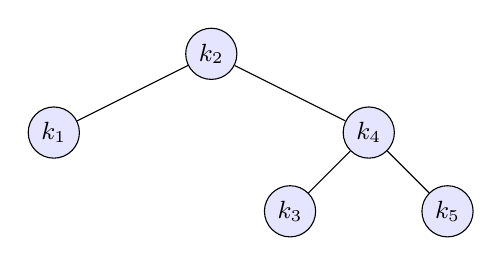
\begin{tikzpicture}[
    level distance=1.0cm,
    level 1/.style={sibling distance=4cm},
    level 2/.style={sibling distance=2cm},
    every node/.style={circle, draw, fill=blue!10,
                       inner sep=2pt, minimum size=0.65cm, font=\small}]
  \node {$k_2$}
    child { node {$k_1$} }
    child { node {$k_4$}
      child { node {$k_3$} }
      child { node {$k_5$} }
    };
\end{tikzpicture}
\end{center}

\begin{center}
\renewcommand{\arraystretch}{1.2}
\begin{tabular}{ccc}
\toprule
$i$ & $\depth_T(k_i)$ & $\depth_T(k_i) \cdot p_i$ \\
\midrule
1 & 1 & 0.25 \\
2 & 0 & 0    \\
3 & 2 & 0.10 \\
4 & 1 & 0.20 \\
5 & 2 & 0.60 \\
\midrule
  &   & $\sum = 1.15$ \\
\bottomrule
\end{tabular}
\end{center}

$E[\text{coût}] = 1 + 1.15 = 2.15$.

\textbf{Arbre B} (racine $k_2$, mais $k_5$ enfant droit de $k_2$, $k_4$ à gauche de $k_5$, $k_3$ à gauche de $k_4$) :

\begin{center}
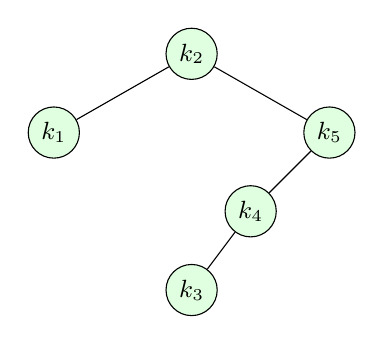
\begin{tikzpicture}[
    level distance=1.0cm,
    level 1/.style={sibling distance=3.5cm},
    level 2/.style={sibling distance=2cm},
    level 3/.style={sibling distance=1.5cm},
    every node/.style={circle, draw, fill=green!12,
                       inner sep=2pt, minimum size=0.65cm, font=\small}]
  \node {$k_2$}
    child { node {$k_1$} }
    child { node {$k_5$}
      child { node {$k_4$}
        child { node {$k_3$} }
        child[missing] {}
      }
      child[missing] {}
    };
\end{tikzpicture}
\end{center}

\begin{center}
\renewcommand{\arraystretch}{1.2}
\begin{tabular}{ccc}
\toprule
$i$ & $\depth_T(k_i)$ & $\depth_T(k_i) \cdot p_i$ \\
\midrule
1 & 1 & 0.25 \\
2 & 0 & 0    \\
3 & 3 & 0.15 \\
4 & 2 & 0.40 \\
5 & 1 & 0.30 \\
\midrule
  &   & $\sum = 1.10$ \\
\bottomrule
\end{tabular}
\end{center}

$E[\text{coût}] = 1 + 1.10 = \mathbf{2.10}$ — cet arbre s'avère être optimal.

\begin{remark}{Observations clés}{obsobs}
\begin{itemize}[noitemsep]
  \item L'OBST n'est \emph{pas} nécessairement l'arbre de hauteur minimale.
  \item La clé de plus grande probabilité n'est \emph{pas} nécessairement à la racine.
  \item Le nombre d'ABR à $n$ nœuds est exponentiel (nombres de Catalan $\sim 4^n/n^{3/2}$),
        donc la force brute est impraticable.
\end{itemize}
\end{remark}

% ─────────────────────────────────────────────────────────────────────────────
\subsection{Sous-structure optimale}

Un ABR se construit en choisissant une racine $k_r$, puis en construisant
récursivement le sous-arbre gauche sur $k_i, \ldots, k_{r-1}$ et le sous-arbre
droit sur $k_{r+1}, \ldots, k_j$.

\begin{theorem}{Sous-structure optimale de l'OBST}{obstopt}
Si l'on construit un ABT optimal sur $k_i, \ldots, k_j$ avec racine $k_r$, alors
les sous-arbres gauche et droit doivent eux aussi être des OBST (sur
$k_i, \ldots, k_{r-1}$ et $k_{r+1}, \ldots, k_j$ respectivement).
\end{theorem}

\textbf{Analyse du coût.} En notant $w(i,j) = \sum_{\ell=i}^{j} p_\ell$ la somme
des probabilités sur $k_i, \ldots, k_j$, on observe que quand un sous-arbre devient
le fils gauche ou droit de la racine, la profondeur de chacun de ses nœuds augmente
de~1. Donc :

\[
  E[\text{coût sous-arbre } k_i \ldots k_j]
  = p_r + \bigl(w(i,r-1) + E[\text{coût gauche}]\bigr)
        + \bigl(w(r+1,j) + E[\text{coût droit}]\bigr).
\]

En regroupant, on obtient :
\[
  E[\text{coût}] = p_r + w(i,r-1) + E[\text{coût gauche}] + w(r+1,j) + E[\text{coût droit}]
                 = w(i,j) + E[\text{coût gauche}] + E[\text{coût droit}].
\]

% ─────────────────────────────────────────────────────────────────────────────
\subsection{Formulation récursive}

Définissons $e[i,j]$ comme le coût de recherche espéré de l'OBST construit sur
$k_i, \ldots, k_j$, et $w(i,j) = \sum_{\ell=i}^{j} p_\ell$.

\[
  e[i, j] =
  \begin{cases}
    0 & \text{si } i = j + 1 \quad (\text{sous-arbre vide}), \\[6pt]
    \displaystyle\min_{i \le r \le j}
      \bigl\{ e[i, r-1] + e[r+1, j] + w(i,j) \bigr\}
    & \text{si } i \le j.
  \end{cases}
\]

On veut calculer $e[1, n]$.

\begin{remark}{Lien avec la somme des probabilités}{wlink}
Le terme $w(i,j) = \sum_{\ell=i}^{j} p_\ell$ peut être précalculé de façon
incrémentale : $w(i,j) = w(i,j-1) + p_j$, ce qui évite de le recalculer à chaque
étape.
\end{remark}

% ─────────────────────────────────────────────────────────────────────────────
\subsection{Algorithme bottom-up}

On remplit les tables $e$ et $r$ (racines optimales) par longueur de chaîne
croissante ($\ell = j - i + 1$ de 1 à $n$) :

\begin{algorithm}[H]
\caption{Optimal-BST($p$, $n$)}
\begin{algorithmic}[1]
\State Créer les tables $e[1\ldots n+1,\; 0\ldots n]$,
       $w[1\ldots n+1,\; 0\ldots n]$ et $r[1\ldots n,\; 1\ldots n]$
\For{$i = 1$ \textbf{to} $n+1$}
    \State $e[i, i-1] \leftarrow 0$     \AlgComment{sous-arbres vides}
    \State $w[i, i-1] \leftarrow 0$
\EndFor
\For{$\ell = 1$ \textbf{to} $n$}        \AlgComment{longueur de la chaîne}
    \For{$i = 1$ \textbf{to} $n - \ell + 1$}
        \State $j \leftarrow i + \ell - 1$
        \State $e[i,j] \leftarrow \infty$
        \State $w[i,j] \leftarrow w[i, j-1] + p_j$
        \For{$r = i$ \textbf{to} $j$}   \AlgComment{essayer chaque racine}
            \State $t \leftarrow e[i, r-1] + e[r+1, j] + w[i,j]$
            \If{$t < e[i,j]$}
                \State $e[i,j] \leftarrow t$
                \State $\mathit{root}[i,j] \leftarrow r$  \AlgComment{mémoriser la racine optimale}
            \EndIf
        \EndFor
    \EndFor
\EndFor
\State \Return $e$ et $\mathit{root}$
\end{algorithmic}
\end{algorithm}

\begin{complexity}{Optimal-BST}{obstcplx}
\begin{itemize}[noitemsep]
  \item La table $e$ contient $O(n^2)$ entrées.
  \item Chaque entrée $e[i,j]$ requiert $O(n)$ pour tester toutes les racines $r$.
  \item \textbf{Complexité totale : $\Theta(n^3)$ en temps, $\Theta(n^2)$ en espace.}
\end{itemize}
\end{complexity}

% ─────────────────────────────────────────────────────────────────────────────
\subsection{Exemple numérique complet}

Avec $p = (0.25,\, 0.2,\, 0.05,\, 0.2,\, 0.3)$, la table $e[i,j]$ remplie
ligne par ligne (indices $j$ en colonnes, $i$ en lignes) :

\begin{center}
\renewcommand{\arraystretch}{1.5}
\begin{tabular}{c|cccccc}
\toprule
$e[i,j]$ & $j=0$ & $j=1$ & $j=2$ & $j=3$ & $j=4$ & $j=5$ \\
\midrule
$i=1$ & 0 & 0.25 & 0.65 & 0.80 & 1.25 & \cellcolor{blue!20}\textbf{2.10} \\
$i=2$ &   & 0    & 0.20 & 0.30 & 0.75 & 1.35 \\
$i=3$ &   &      & 0    & 0.05 & 0.30 & 0.85 \\
$i=4$ &   &      &      & 0    & 0.20 & 0.70 \\
$i=5$ &   &      &      &      & 0    & 0.30 \\
$i=6$ &   &      &      &      &      & 0    \\
\bottomrule
\end{tabular}
\end{center}

L'OBST a un coût de recherche espéré de $e[1,5] = \mathbf{2.10}$.

\textbf{Calcul de $e[1,2]$ pour illustration :}
$w(1,2) = p_1 + p_2 = 0.45$. On teste :
\begin{itemize}[noitemsep]
  \item $r = 1$ : $e[1,0] + e[2,2] + 0.45 = 0 + 0.20 + 0.45 = 0.65$
  \item $r = 2$ : $e[1,1] + e[3,2] + 0.45 = 0.25 + 0 + 0.45 = 0.70$
\end{itemize}
Minimum : $e[1,2] = 0.65$ avec $r = 1$ (racine $k_1$).

% ─────────────────────────────────────────────────────────────────────────────
\subsection{Reconstruction de l'arbre optimal}

La table $\mathit{root}[i,j]$ mémorise la racine choisie à chaque étape. On
reconstruit l'arbre récursivement :

\begin{algorithm}[H]
\caption{Build-Optimal-BST($\mathit{root}$, $i$, $j$, $\mathit{parent}$)}
\begin{algorithmic}[1]
\If{$i > j$}
    \State \Return \AlgComment{sous-arbre vide}
\EndIf
\State $r \leftarrow \mathit{root}[i,j]$
\State \textbf{afficher} ``$k_r$ est \{racine / fils gauche / fils droit\} de $\mathit{parent}$''
\State \Call{Build-Optimal-BST}{$\mathit{root}$, $i$, $r-1$, $k_r$}   \AlgComment{sous-arbre gauche}
\State \Call{Build-Optimal-BST}{$\mathit{root}$, $r+1$, $j$, $k_r$}   \AlgComment{sous-arbre droit}
\end{algorithmic}
\end{algorithm}

% ─────────────────────────────────────────────────────────────────────────────
\subsection{Résumé : OBST}

\begin{tcolorbox}[colback=lightblue, colframe=keyblue, fonttitle=\bfseries,
                  title={Récapitulatif DP – Arbre Binaire de Recherche Optimal}]
\begin{itemize}[noitemsep]
  \item \textbf{Choix} : quelle clé $k_r$ placer à la racine du sous-arbre
        $k_i, \ldots, k_j$.
  \item \textbf{Sous-structure optimale} : les sous-arbres gauche et droit
        doivent eux-mêmes être des OBST.
  \item \textbf{Récurrence} :
    \[
      e[i,j] =
      \begin{cases}
        0 & i = j+1,\\
        \displaystyle\min_{i \le r \le j}
          \bigl\{e[i,r-1] + e[r+1,j] + w(i,j)\bigr\} & i \le j.
      \end{cases}
    \]
  \item \textbf{Complexité} : $\Theta(n^3)$ en temps, $\Theta(n^2)$ en espace.
  \item \textbf{Reconstruction} : table $\mathit{root}[i,j]$ + appels récursifs.
\end{itemize}
\end{tcolorbox}

% ─────────────────────────────────────────────────────────────────────────────
\subsection{Tableau récapitulatif général de la DP}

\begin{center}
\renewcommand{\arraystretch}{1.45}
\begin{tabular}{llcc}
\toprule
\textbf{Problème} & \textbf{Choix} & \textbf{Complexité} & \textbf{Table} \\
\midrule
Coupe de tiges      & Position de la coupe gauche        & $\Theta(n^2)$  & $n+1$ \\
Rendu de monnaie    & Dénomination utilisée              & $O(nW)$        & $W+1$ \\
Chaînes de matrices & Position de la parenthèse          & $\Theta(n^3)$  & $n^2$ \\
LCS                 & Inclure $x_i = y_j$ / avancer      & $\Theta(mn)$   & $(m+1)(n+1)$ \\
OBST                & Racine du sous-arbre $k_i\ldots k_j$ & $\Theta(n^3)$& $n^2$ \\
\bottomrule
\end{tabular}
\end{center}